
% This LaTeX was auto-generated from an M-file by MATLAB.
% To make changes, update the M-file and republish this document.

\documentclass{article}
\usepackage{graphicx}
\usepackage{color}

\sloppy
\definecolor{lightgray}{gray}{0.5}
\setlength{\parindent}{0pt}

\begin{document}

    
    
\subsection*{Contents}

\begin{itemize}
\setlength{\itemsep}{-1ex}
   \item spatial domain
   \item frequency domain
\end{itemize}
\begin{verbatim}
close all;
[gifImage cmap] = imread('octone.gif');
im = ind2rgb(gifImage, cmap);

% original image
figure;
imshow(im);

%convert white region to black
im(im(:,:,3) == 1) = 0;
\end{verbatim}

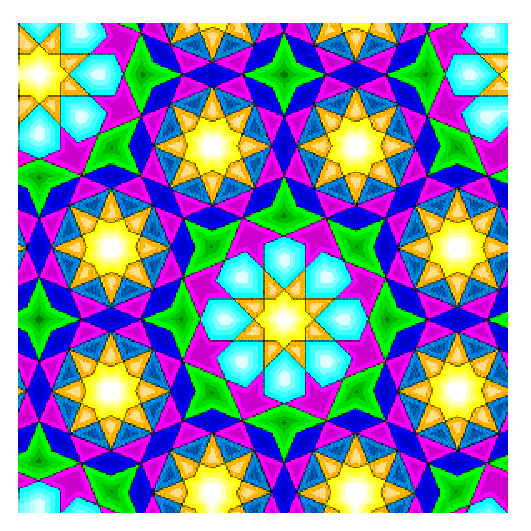
\includegraphics [width=4in]{yellow2_01.eps}


\subsection*{spatial domain}

\begin{verbatim}
out1 = im(:,:,1);
out2 = im(:,:,2);

% Multiplication of red and green channel outputs non-zero only for yellow
% portion and 0 for all other portions
out3 = out1.*out2;

%display all the yellow shade stars
figure;
imshow(mat2gray(out3));

%display only pure yellow stars
out3(out3 < 1) = 0;
figure;
imshow(mat2gray(out3));
\end{verbatim}

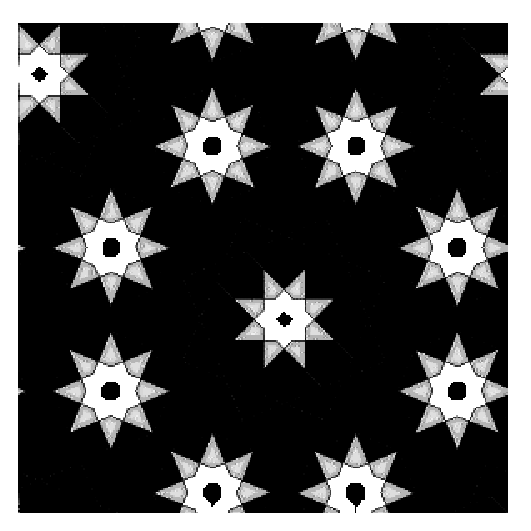
\includegraphics [width=4in]{yellow2_02.eps}

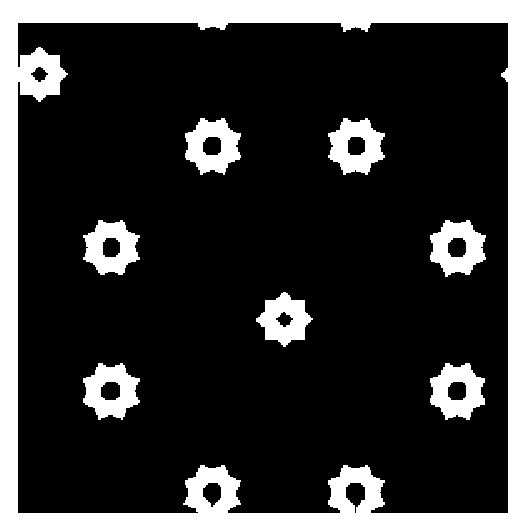
\includegraphics [width=4in]{yellow2_03.eps}


\subsection*{frequency domain}

\begin{verbatim}
%multiplication in spatial domain is convolution in frequency domain
C = real(ifft2(fftshift(conv2(fftshift(fft2(out1)),(fftshift(fft2(out2)))))));

%scale the intensity values to lie between 0 and 255
C = (C-min(C(:)))*255/(max(C(:)) - min(C(:)));

%display all the yellow shade stars
figure;
imshow(imresize(C,[size(im,1) size(im,2)]),[]);

%display only pure yellow stars
C(C < 0.64*max(C(:))) = 0;
figure;
imshow(imresize(C,[size(im,1) size(im,2)]),[]);
\end{verbatim}

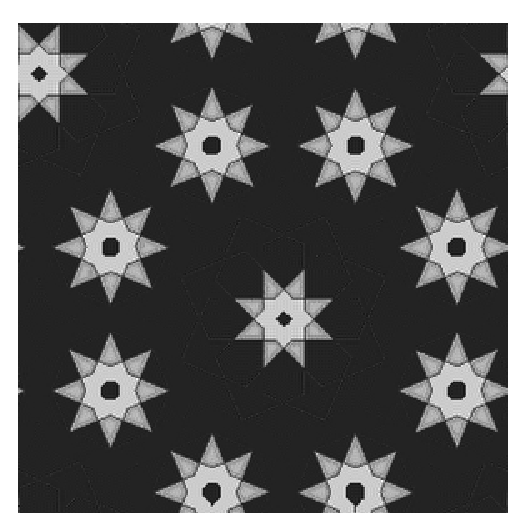
\includegraphics [width=4in]{yellow2_04.eps}

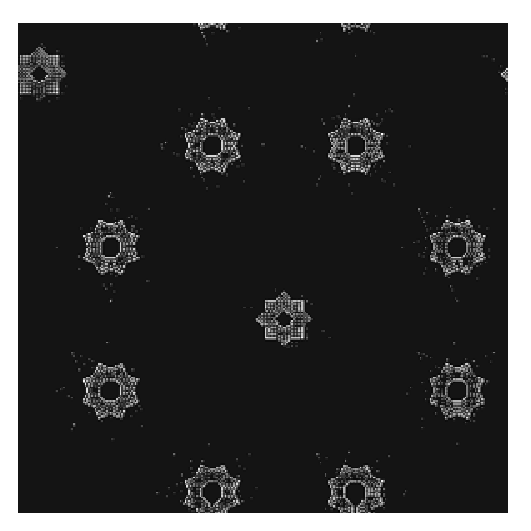
\includegraphics [width=4in]{yellow2_05.eps}



\end{document}
    
